\documentclass[a4paper, 11pt]{article}
\usepackage[polish]{babel}
\usepackage[MeX]{polski}
\usepackage[utf8]{inputenc}
\usepackage[T1]{fontenc}
%\usepackage{times}
\usepackage{graphicx,wrapfig}
%\usepackage{anysize}
%\usepackage{tikz}
%\usetikzlibrary{calc,through,backgrounds,positioning}
\usepackage{anysize}
\usepackage{float}
\usepackage{adjustbox}
%\usepackage{stmaryrd}
%\usepackage{amssymb}
%\usepackage{amsthm}
%\marginsize{3cm}{3cm}{3cm}{3cm}
%\usepackage{amsmath}
%\usepackage{color}
%\usepackage{listings}
%\usepackage{enumerate}
%\lstloadlanguages{Ada,C++}


\begin{document}	
	% \noindent -  w tym akapicie nie bedzie wciecia
	% \ indent - to jest aut., ale powoduje ze jest wciecie
	% \begin{flushleft}, flushright, center - wyrownianie akapitu
	% \textbf{pogrubiany tekst}
	% \textit{kursywa} 
	% 					STRONY 
	%  http://www.codecogs.com/latex/eqneditor.php 
	%  http://www.matematyka.pl/latex.htm
	% 
	\begin{titlepage}
		
		
		
		\newcommand{\HRule}{\rule{\linewidth}{0.5mm}} % Defines a new command for the horizontal lines, change thickness here
		
		\center % Center everything on the page
		
		%----------------------------------------------------------------------------------------
		%	HEADING SECTIONS
		%----------------------------------------------------------------------------------------
		
		\textsc{\LARGE Akademia Górniczo-Hutnicza im. Stanisława Staszica}\\[1.5cm] % Name of your university/college
		\textsc{\Large Kraków}\\[0.5cm] % Major heading such as course name
		\textsc{\large }\\[0.5cm] % Minor heading such as course title
		
		%----------------------------------------------------------------------------------------
		%	TITLE SECTION
		%----------------------------------------------------------------------------------------
		
		\HRule \\[0.4cm]
		{\fontsize{38}{50}\selectfont Bankomat}
		%	{ \Huge \bfseries} Osadnicy z Catan - Gra sieciowa\\[0.3cm] % Title of your document
		\HRule \\[1.5cm]
		
		%----------------------------------------------------------------------------------------
		%	AUTHOR SECTION
		%----------------------------------------------------------------------------------------
		
		% If you don't want a supervisor, uncomment the two lines below and remove the section above
		\Large \emph{Autorzy:}\\
		Katarzyna \textsc{Kosiak} \\
		Joanna \textsc{Roczniak}\\[3cm]\ % Your name
		
		
		%----------------------------------------------------------------------------------------
		%	DATE SECTION
		%----------------------------------------------------------------------------------------
		
		{\large \today}\\[3cm] % Date, change the \today to a set date if you want to be precise
		
		%----------------------------------------------------------------------------------------
		%	LOGO SECTION
		%----------------------------------------------------------------------------------------
		
		%\includegraphics{Logo}\\[1cm] % Include a department/university logo - this will require the graphicx package
		
		%----------------------------------------------------------------------------------------
		
		\vfill % Fill the rest of the page with whitespace
		
	\end{titlepage}
	
	%SPIS TRESI
	%
	%
	%
	%
	%
	%
	%
	%
	%
	
	\tableofcontents
	\vfill
	\newpage	%\pagebreak
	
	%SEKCJE
	%opis zagadnienia, temat, problem, dlaczego chcemy to rozwiązacyać metodą ewolucyjnę
	%jakie są metody rozwiącania problemu, przegląd literatury,
	%proponowane rozwiązania (spójność)
	%czym się inspierowałyśmy
	%
	%
	%
	
	%\setlength{\parskip}{1ex plus 0.5ex minus 0.2ex}
	
	\section{Wstęp}
	\indent
	
	Niniejszy dokument stanowi dokumentację projektu ``Bankomat'' z przedmiotu Analiza i modelowanie oprogramowania.
	
	\section{Opis}
		\indent
		
	Bankomat - automatyczne urządzenie służące przede wszystkim do wyplaty gotówki za pomocą magnetycznej lub inteligentnej (mikroprocesorowej, chipowej) karty płatniczej. Bankomat służy także do drukowania potwierdzeń i dostarczania informacji o stanie konta.
	
	Działanie bankomatu opiera się  na systemie informatycznym umożliwiającym wymianę informacji z tzw. systemem autoryzacyjnym. Na podstawie informacji zawartych na karcie płatniczej i osobistego, poufnego numeru identyfikacyjnego klienta (tzw. PIN-u), zapobiegającego użyciu tej karty przez osobę niebędącą właścicielem bądź zezwalającego na użycie jej przez osobę upoważnioną przez właściciela karty bankomat łączy się z systemem autoryzacyjnym i po otrzymaniu komunikatu zwrotnego wyrażającego zgodę na wykonanie żądanej operacji, realizuje ją. Operacją taką może być wypłata  gotówki, wydruk potwierdzenia i sprawdzenie stanu rachunku.
	
	W przypadku utraty pełnej funkcjonalności przez bankomat osoby uprawnione mogą uzyskać do niego specjalny dostęp w celu naprawy lub dołożenia gotówki.
	
	\section{Analiza wymagań}
	\indent
		
	\begin{minipage}[t]{0.8\textwidth}                          % minipage spans half the textwidth
		\begin{center}
			\begin{adjustbox}{center, width=\columnwidth}     	
		
		
	\begin{tabular}{|c|c|c|c|c|}
		\hline ID & OPIS & PRIORYTET & KRYTYCZNOŚĆ & HARMONOGRAM  \\ 
		\hline R01 & Wydawanie pieniędzy & Wysoki & Wysoka & Release 1 \\ 
		\hline R02 & Sprawdzenie stanu konta &  Wysoki & Średnia &  Release 1  \\ 
		\hline  R03 & Naprawa maszyny &  Wysoki & Wysoka &  Release 1  \\ 
		\hline  R04 & Dostęp techniczny dla osób upoważnionych &  Wysoki & Wysoka &  Release 1  \\ 
		\hline 
	\end{tabular} 
		
		
\end{adjustbox}
\end{center}
\end{minipage}		
		
		
	
	\section{Diagramy przypadków użycia}
	\indent
		
	\begin{figure}[H]%[!htb]
			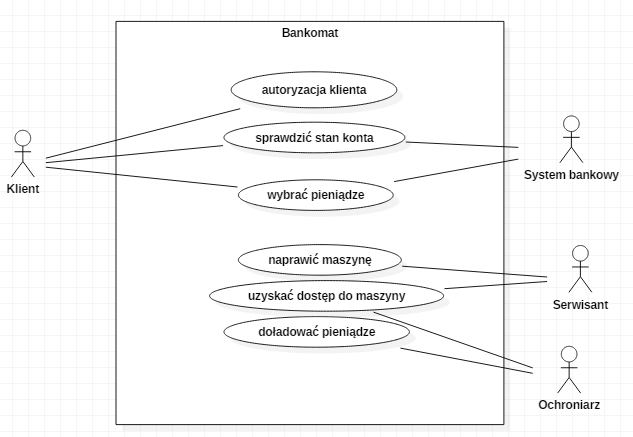
\includegraphics[scale=1.0]{usecase1.png}\caption{Ogólny diagram przypadków użycia}
	\end{figure}
	
	\begin{figure}[H]%[!htb]
			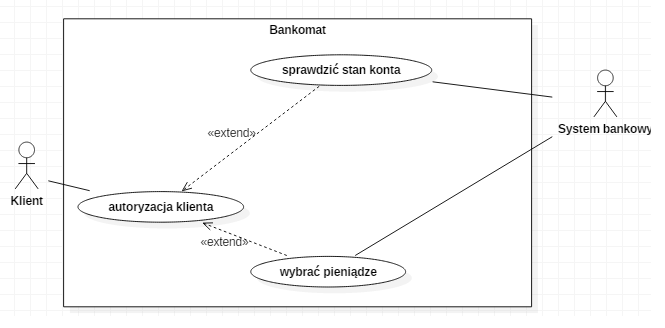
\includegraphics[scale=0.9]{usecase2.png}\caption{Diagram przypadków użycia - autoryzacja}
	\end{figure}
	
	\begin{figure}[H]%[!htb]
			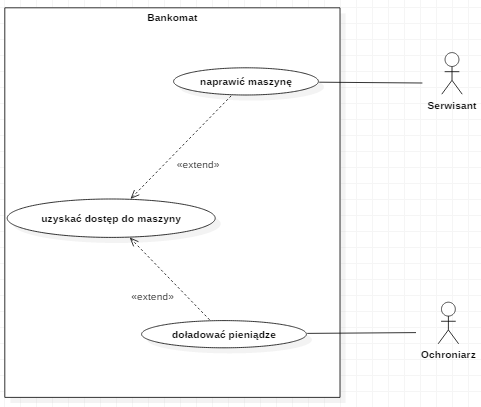
\includegraphics[scale=1.0]{usecase3.png}\caption{Diagram przypadków użycia -serwisant i ochroniarz}
	\end{figure}
		
	\section{Diagram sekwencji}
	\indent
			
	\begin{figure}[H]%[!htb]
			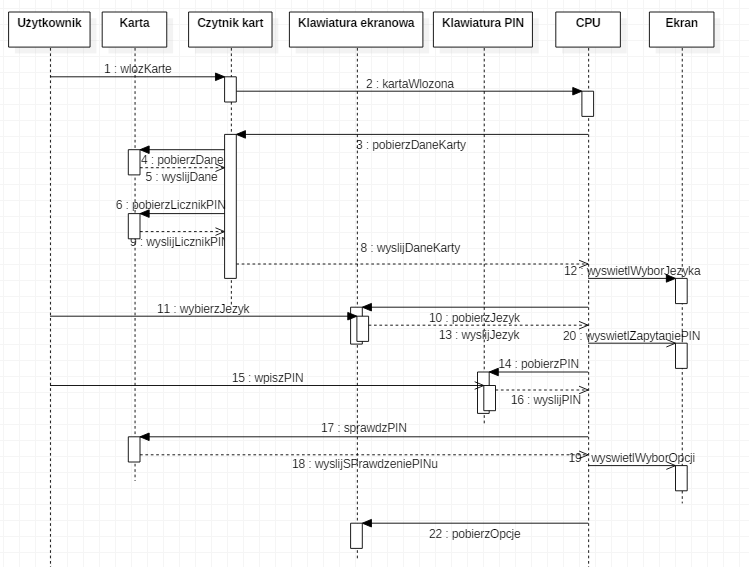
\includegraphics[scale=0.9]{sequence1.png}\caption{Diagram sekwencji - autoryzacja}
	\end{figure}
	
	\begin{figure}[H]%[!htb]
			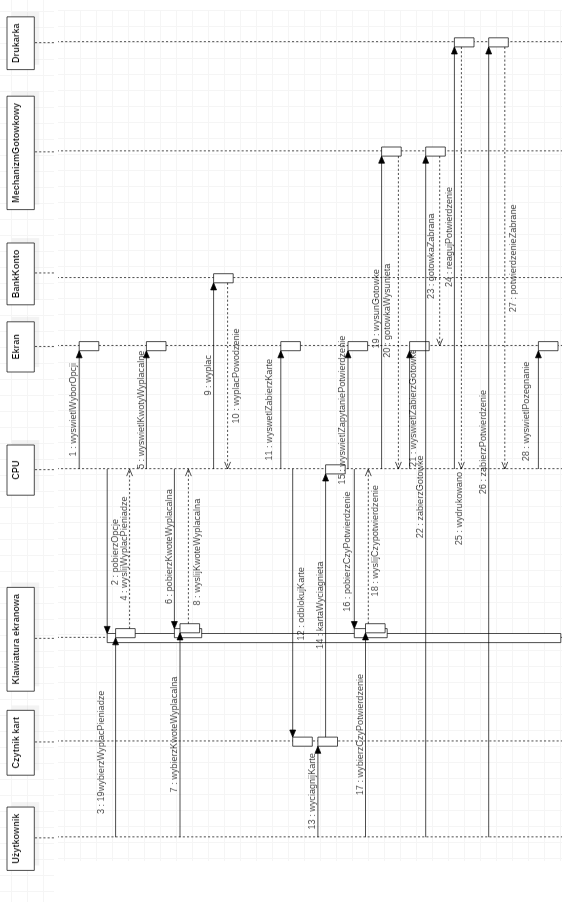
\includegraphics[scale=0.9]{sequence2.png}\caption{Diagram sekwencji - wypłata pieniedzy}
	\end{figure}
	
	\begin{figure}[H]%[!htb]
			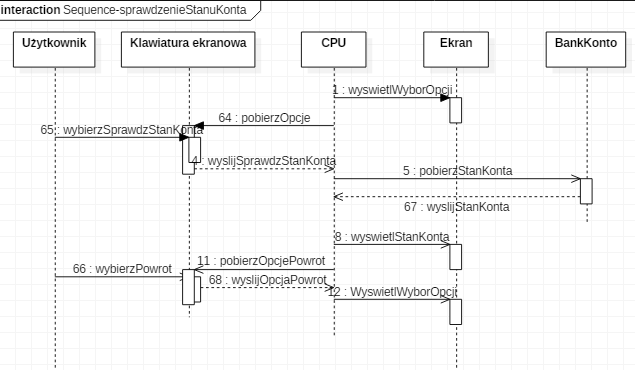
\includegraphics[scale=0.9]{sequence3.png}\caption{Diagram sekwencji -sprawdzenie stanu konta}
	\end{figure}
	
	\begin{figure}[H]%[!htb]
		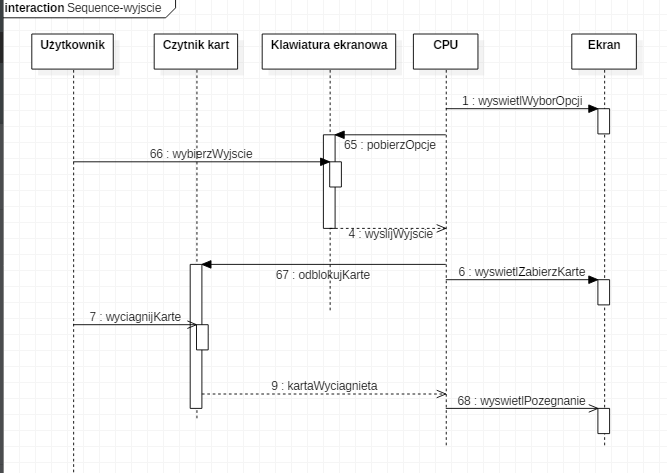
\includegraphics[scale=0.9]{sequence4.png}\caption{Diagram sekwencji - wyjście}
	\end{figure}
		
	
	
	
	
\end{document}
